\chapter{Background}
\label{sec:background}

This chapter provides an overview of the fundamental concepts and techniques that form the background for this dissertation.

\section{Classical Planning}
\label{sec:classical-planning}

Tipically we provide a formal description of the problem to find a solution from search algorithms. In classical planning, a problem is represented as a planning task. We define the various concepts that constitute a planning task, which are addressed throughout the dissertation.

\begin{definition}{Fact}
    \label{def:fact}
    A fact $f$ is a statement that represents a condition or characteristic of the environment and can be either true or false.
\end{definition}

Typically, a domain has a set of facts denoted as~$\mathcal{F} = \{f_1, \ldots, f_n\}$. For example, consider the domain VisitAll, where a robot explores a grid and aims to visit all its cells. In this scenario, facts can be used to represent the robot's position and the status of each cell, indicating whether it has been visited or not. Consider a grid with 2~cells labeled~$c0$ and $c1$. In this case, the set of facts can be represented as~$\mathcal{F} = \{\text{at-robot}(c0),\text{at-robot}(c1),\text{visited}(c0),\text{visited}(c1)\}$.

\begin{definition}{Mutex}
    \label{def:mutex}
    A mutex~(mutual exclusion) is a condition where two or more facts cannot occur simultaneously.
\end{definition}

In VisitAll, the robot cannot be in two positions simultaneously. Therefore, the set of facts~$\{\text{at-robot}(c0),\text{at-robot}(c1)\}$ represents a mutex.

\begin{definition}{Variable}
    \label{def:variable}
    A variable~$v$ is a concise representation of a condition or characteristic of the environment. It can assume any value from a predefined domain~$D(v)$.
\end{definition}

A variable groups a collection of mutually exclusive facts, where each fact corresponds to a value~$d \in D(v)$ that can be assigned to the variable~$v$ at any given moment, allowing for a single assignment at a time. (Note that a mutex can also arise between values of different variables.) For instance, in the VisitAll domain, all the facts representing the robot's position can be combined into a variable. This approach significantly reduces the size required to represent the robot's position. Instead of necessitating $n$~facts in a grid with $n$~cells, we have a single variable~$v_p$ with $|D(v_p)| = n$. Similarly to facts, each domain has a set of variables~$\mathcal{V} = \{v_1,\ldots,v_n\}$.

\begin{definition}{State}
    \label{def:state}
    A state~$s$ is an assignment of all variables~$v \in \mathcal{V}$.
\end{definition}

A state where all variables are defined is also called a complete state. When the set of variables is not fully assigned, i.e.,~one or more variables~$v \in \mathcal{V}$ do not have a defined value~$d \in D(v)$, it is a partial state. Let $s(v)$ be the value of variable~$v$ in state~$s$. The value of an undefined variable~$v$ is written as~$s(v) = \bot$. We say that $s \subseteq t$ if $s(v) = t(v)$ for all $v \in \mathcal{V}$ such that $t(v) \neq \bot$. This implies that there is an assignment of undefined variables such that $s = t$. Therefore, a partial state~$t$ represents a set of states containing every state whose $s \subseteq t$. The initial state~$s_0$ is a complete state that corresponds to the initial variable assignment. The goal $s^*$ is defined as a partial state.

\begin{definition}{Operator}
    \label{def:operator}
    An operator~$o$, also known as action, is defined as a pair of preconditions and effects~$(\pre(o),\eff(o))$, both partial states. The preconditions specify the conditions that must hold in the current state for an operator to be applicable, while the effects describe the changes in the state that occur when the operator is applied.
\end{definition}

Let $\mathcal{O}$ be the set of all operators in a given task. An operator~$o \in \mathcal{O}$ is applicable to a state~$s$ if $s \subseteq \pre(o)$, and produces a successor state~$s' = \sucs(s,o) := \eff(o) \circ s$, where $s'~=~t~\circ~s$ is defined by $s'(v) = t(v)$ for all $v$ such that $t(v)$ is defined, and $s'(v)=s(v)$ otherwise. The set of all successor states of state~$s$ is $\sucs(s) = \{\sucs(s,o) \mid o \in \mathcal{O}, s \subseteq \pre(o)\}$. Each operator is assigned a cost based on the mapping function~$cost:\mathcal{O}\rightarrow\R_{+}$; when the cost is omitted, it assumes a unit cost, i.e.,~$cost(o) = 1$ for each operator~$o \in \mathcal{O}$.

A sequential application of operators is called a progression. Alternatively, a regression is a backward sequential application of operators. For regression, we consider an operator~$o$ to be relevant for partial state~$s$ if $\eff_r=\dom(\eff(o))\cap\dom(s)\neq\emptyset$; the operator is consistent if $s \subseteq \eff(o)|_{\eff_r}$. Relevance requires at least one defined effect in the partial state to be regressed, consistency, and an agreement on defined effects. An operator~$o$ then is backward applicable in partial state~$s$ if it is relevant and consistent with~$s$ and leads to predecessor $r=\pre(o)\circ (s|_{\dom(s)\setminus\eff_r})$. Note that $s \subseteq \sucs(r,o)$, but may differ from~$s$. Similar to progression, a partial state~$s$ has predecessors $\pred(s)=\{\pred(s,o)\mid o\in \mathcal{O}, \text{o backward applicable to }s\}$. A regression sequence from state~$s_0$ then is valid if $o_i$ can be applied to~$s_{i-1}$ and produces~$s_i=\pred(s_{i-1},o_i)$. All partial states~$s_k$ can reach a partial state~$s_0 \subseteq s$ in at most~$k$ forward applications of the reversed operator sequence.

\begin{definition}{Plan}
    \label{def:plan}
    A plan is a sequence of operators $\pi=(o_1,\ldots,o_k)$.
\end{definition}

A plan is valid for state~$s_0$, referred to as an $s_0$-plan, if for $i\in[k]$ operator~$o_i$ can be applied to $s_{i-1}$ and produces $s_i=\sucs(s_{i-1},o_i)$, where $s_k \subseteq s^*$. The cost of plan~$\pi$ is $\sum_{i\in[k]} \text{cost}(o_i)$. When a plan has the lowest cost among all $s_0$-plans, it is called an optimal plan.

\begin{definition}{State Space}
    \label{def:statespace}
    A state space is the set of all the states over the variables~$v \in \mathcal{V}$.
\end{definition}

The forward state space (FSS) is the set of all the states reachable from initial state~$s_0$ by applying a sequence of operators. Similarly, the backward state space (BSS) is the set of all the partial states reachable from the goal~$s^*$ by applying a sequence of backward operators.

\subsection{STRIPS Representation}
\label{sec:strips}

The STRIPS (Stanford Research Institute Problem Solver) representation~\cite{fikes1971strips} is a fundamental approach used in planning tasks to model and reason about the state of the environment. In this representation, a planning task is defined by a set of predicates (facts) that describe the various attributes and conditions of the problem domain. Each fact represents a specific property that can be true or false in a given state. The preconditions and effects of operators are expressed as a set of facts.

\begin{definition}{STRIPS Planning Task}
    \label{def:strips}
    A STRIPS planning task is defined as a tuple~$\Pi=\langle\mathcal{F},\mathcal{O},s_0,s^*, \text{cost}\rangle$, where $\mathcal{F}$~is a set of facts, $\mathcal{O}$~is a set of operators over $\mathcal{F}$, $s_0$~an initial state, $s^*$~the goal condition, and $\text{cost}:\mathcal{O}\rightarrow\R_{+}$~a function mapping operators to costs.
\end{definition}

Throughout this dissertation, we present samples represented in the STRIPS formalism. The motivation behind this approach lies in the compatibility between the propositional nature of STRIPS, where facts can be either true or false, and the proposed neural network input in binary format, which is more suitable for training~(\cref{sec:learning-heuristics}). Additionally, the Fast~Downward planning system used in this dissertation incorporates PDDL~(Planning Domain Definition Language) as its input language. PDDL provides a formal and widely accepted syntax for describing planning tasks in the STRIPS representation.

\begin{figure}[tb]
    \caption{VisitAll domain description in PDDL.}
    \label{fig:pddl}
    \centering
    \begin{lstlisting}[basicstyle=\ttfamily]
        (define (domain grid-visit-all)
            (:requirements :typing)
            (:types place - object)
            (:predicates (connected ?x ?y - place)
                        (at-robot ?x - place)
                        (visited ?x - place))
            (:action move
                :parameters (?curpos ?nextpos - place)
                :precondition (and
                    (at-robot ?curpos)
                    (connected ?curpos ?nextpos))
                :effect (and 
                    (at-robot ?nextpos)
                    (not (at-robot ?curpos))
                    (visited ?nextpos)))
        )
    \end{lstlisting}
    Source: International Planning Competition (IPC) 2014.
\end{figure}

\cref{fig:pddl} shows an example of a domain description in PDDL. The VisitAll domain represents a scenario where a robot navigates a grid and marks each cell it steps on as visited. The objective of this domain is typically to visit all cells in the grid. The initial and goal states are described in a second file, the problem PDDL, along with the object declarations. The domain PDDL specifies the predicates and actions~(operators). In the VisitAll example, we have one object type~(place), three predicates~(connected, at-robot, and visited), and one action~(move). The combination of predicates with objects forms the facts in a process called grounding. For instance, in a grid with two connected cells, $c1$~and~$c2$, we have the set of facts~$\mathcal{F}=\{$connected$(c1,c2)$, \mbox{connected$(c2,c1)$}, \mbox{at-robot$(c1)$}, \mbox{at-robot$(c2)$}, \mbox{visited$(c1)$}, visited$(c2)\}$.

\subsection{\sas Representation}
\label{sec:sasplus}

Another approach to modeling planning tasks is using the \sas representation \cite{backstrom1995complexity}. Although Fast~Downward takes propositional representation with PDDL as its input, internally, it uses finite domains to represent states. The \sas representation enhances the capabilities of a propositional representation by using finite domains~$D$, which explicitly define the possible values for each variable. This enables a more compact and structured representation of the problem.

\begin{definition}{\sas Planning Task}
    \label{def:sasplus}
    A~\sas planning task is defined as a tuple~$\Pi=\langle\mathcal{V},\mathcal{O},s_0,s^*, \text{cost}\rangle$, where $\mathcal{V}$~is a set of variables, $\mathcal{O}$~is a set of operators over $\mathcal{V}$, $s_0$~an initial state, $s^*$~the goal condition, and $\text{cost}:\mathcal{O}\rightarrow\R_{+}$~a function mapping operators to costs.
\end{definition}

\sas and STRIPS differ in their method of representing states and can be converted between each other. For example, consider the VisitAll domain depicted in \cref{fig:pddl}, specifically the at-robot predicate. In PDDL, the action always replaces one robot position with another. Thus, \sas represents this predicate using a variable~$v$ and a value~$d \in D(v)$ for each possible robot position. Consequently, in large grids with hundreds of positions where propositional representation would require many facts, \sas efficiently represents them using a single variable.

\section{Search Algorithms}
\label{sec:search-algorithms}

Search algorithms enable exploring the state space to find a solution for a planning task. They systematically traverse the state space of a problem, aiming to reach the goal from an initial state. Blind search algorithms, in particular, operate without any knowledge about the problem domain and rely solely on the problem representation to guide the search. On the other hand, heuristic search incorporates problem-specific knowledge. It uses heuristics, which are approximate or informed estimates of the cost or distance to the goal, to prioritize exploring more promising paths. The following sections present both approaches.

\subsection{Blind Search}
\label{sec:blind-search}

By exploring the state space exhaustively, blind search algorithms navigate across various states and paths to find potential solutions. An example of a blind search algorithm is the Breadth-First Search~(BFS). BFS explores the state space by systematically expanding all the states at the same distance from the initial state before moving to the next distance. This strategy ensures that the shortest path to a goal state is found. However, BFS can be memory-intensive as it maintains a queue of all the generated but not expanded states in memory.

Depth-First Search~(DFS) also performs a blind search. In DFS, the search starts from an initial state and explores the state space by iteratively expanding the farthest state from the initial state that has not been expanded yet. This algorithm is memory-efficient as it only needs to keep track of a single path from the initial state to the current state. However, DFS does not guarantee an optimal solution and can get trapped in deep branches of the state space.

\begin{figure}[tb]
    \caption[Graph representing a state space.]{Graph representing a state space where the vertices and arcs correspond to states and applicable operators, respectively.}
    \label{fig:statespace}
    \addmargin
    \centering
    \begin{tikzpicture}[every node/.style={circle, draw}, node distance=23mm, minimum size=9mm]
    \node (s0) {$s_0$};
    \node[above right of=s0] (s1) {$s_1$};
    \node[right of=s0] (s2) {$s_2$};
    \node[below right of=s0] (s3) {$s_3$};
    \node[right of=s1] (s4) {$s_4$};
    \node[right of=s2] (s5) {$s_5$};
    \node[right of=s3] (s6) {$s_6$};
    \node[right of=s5] (s7) {$s_7$};
    \node[right of=s6] (s8) {$s_8$};
    \node[above right of=s7] (s9) {$s_9$};
    \node[right of=s7] (s10) {$s_{10}$};
    \node[right of=s8] (s11) {$s_{11}$};
    \node[left of=s9] (goal) {$s^*$};

    \draw[-Straight Barb] (s0) to (s2);
    \draw[-Straight Barb] (s0) to[bend left=5] (s1);
    \draw[-Straight Barb] (s0) to[bend right=5] (s3);
    \draw[-Straight Barb] (s1) to (s4);
    \draw[-Straight Barb] (s2) to (s5);
    \draw[-Straight Barb] (s2) to[bend right=5] (s6);
    \draw[-Straight Barb] (s3) to (s6);
    \draw[-Straight Barb] (s4) to[bend right=5] (s2);
    \draw[-Straight Barb] (s5) to (s7);
    \draw[-Straight Barb] (s7) to[bend left=5] (s8);
    \draw[-Straight Barb] (s7) to[bend left=5] (s9);
    \draw[-Straight Barb] (s7) to (s10);
    \draw[-Straight Barb] (s8) to (s6);
    \draw[-Straight Barb] (s9) to (goal);
    \draw[-Straight Barb] (s10) to[bend left=5] (s11);
\end{tikzpicture}

\end{figure}

To illustrate, \cref{fig:statespace} presents a state space. BFS starts by expanding the initial state~$s_0$ and then expands $s_1$, $s_2$, and $s_3$. In sequence, it expands the successor of $s_1$ ($s_4$), then of $s_2$ ($s_5$ and $s_6$), until a solution is found. On the other hand, DFS expands the initial state~$s_0$ and continues expanding a newly generated successor until it reaches a solution or a state without successors (e.g.,~$s_6$ or $s_{11}$), at which point the algorithm backtracks to the nearest state that has an unexpanded successor and continues the search.

Blind search algorithms are unsuitable for solving planning tasks due to their lack of efficiency in exploring the state space, which is typically vast and contains numerous paths. Instead, heuristic search is used, which will be introduced in the next section. However, BFS and DFS can still be valuable in planning as sampling algorithms. By sampling the state space using these algorithms, we can selectively focus on regions either closer to the initial state, using BFS, or, more distant, using DFS.

\subsection{Heuristic Search}
\label{sec:heuristic-search}

Exploring the state space systematically to find a plan can quickly become computationally infeasible for planning domains with large state spaces. Therefore, the primary approach for solving planning tasks is heuristic search. Heuristic search algorithms address this challenge by using heuristics to guide the search toward promising regions of the state space. These heuristics estimate how close a given state is to a goal state and guide which successors to prioritize during the search.

A commonly used heuristic search algorithm in classical planning is \astar search. \astar combines the cost of reaching a state from the initial state~($g$-value) with a heuristic estimate of the remaining cost to reach the goal~(\h-value). By considering both the past cost and the estimated future cost, \astar can efficiently explore the state space to find the optimal solution, provided that the heuristic is admissible~(does not overestimate the actual \h-value).

Greedy Best-First Search~(GBFS), another widely used heuristic search algorithm in classical planning, is a variant of \astar search that prioritizes expanding states with the lowest heuristic values without considering the past cost of reaching those states. Both \astar and GBFS are considered a ``greedy'' algorithm because it only considers the heuristic estimate and makes decisions solely based on that information. While GBFS can be highly efficient regarding exploration speed, it does not guarantee finding an optimal solution as \astar does. Nonetheless, GBFS is a popular choice in planning tasks where finding any feasible solution quickly is more important than finding the optimal solution. Therefore, in our experiments, GBFS serves as the search algorithm.

\subsubsection{Heuristic Functions}
\label{sec:heuristic-functions}

Heuristic search algorithms require the use of a heuristic function. A heuristic function~$h:\mathcal{S}\rightarrow\R_{+}\cup\{\infty\}$ maps each state in the state space~$\mathcal{S}$ to a non-negative number or $\infty$. The number represents the cost-to-goal estimate~(\h-value) for the given state. An infinity value indicates a dead-end state, i.e.,~without any paths leading to the goal. A heuristic function is more efficient when its \h-value closely approximates the actual goal distance. The optimal heuristic \hstar produces the cost of an optimal $s$-plan for all state~$s \in \mathcal{S}$.

The heuristic function has certain properties, such as admissibility, consistency, and goal-awareness. An admissibility heuristic function never overestimates the actual goal distance. It guarantees optimality when combined with specific search algorithms such as \astar. A heuristic function is consistent if, for every state~$s \in \mathcal{S}$ and for every applicable operator~$o$ with $s' = \sucs(s,o)$, it holds that $h(s) \leq cost(o) + h(s')$. Finally, a goal-aware heuristic guarantees $h(s) = 0$ for all goal states~$s \subseteq s^*$.

Heuristics can be arbitrary functions, allowing for flexibility in designing based on domain knowledge and problem-specific insights. Therefore, a heuristic can be classified as model-based or model-free. In a model-free setting, we interact with the planning task only by functions that allow accessing the initial state~$s_0$, the goal condition~$s^*$, and the successors~$\sucs(s)$ of a state $s$. In this setting, we do not have access to the logical description of operators; we only have access to black-box functions~\cite{sturtevant2019exponential} -- which could also be learned~-- that, given a state, returns its successors and predecessors\mr{is that so? could be very costly, mostly not polynomial: there can be many preconditions; a more reasonable model allows to enumerate or sample them}. Note that this setting is also used in reinforcement learning.
% Some approaches\mr{give an example} also provide access to each variable's domain.
In contrast, a model-based heuristic uses the complete description of the model, which permits, for example, reasoning about operators and the computation of mutexes.

An example of a model-based heuristic is the FF~(Fast-Forward) heuristic~\cite{hoffmann2001ff}, which computes its cost-to-goal estimates by considering a relaxed version of the planning problem. In a relaxed version, all effects that remove facts from a state~(delete effects) of the operators are ignored, resulting in a simplified version of the problem. The FF~heuristic extracts a solution from a relaxed version and computes the cost of operators in the plan, using it as the cost-to-goal estimate. As model-free, we have the goal-count heuristic, which does not rely on the planning model. Instead, it counts the number of unsatisfied goal conditions in the current state, assuming that each unsatisfied condition requires an additional unit cost operator to be satisfied. Both the FF and goal-count heuristics are addressed in our experiments~(\cref{sec:experiments}).

\section{Neural Networks}
\label{sec:neural-networks}

Neural networks~(NN) have gained popularity due to their ability to learn and generalize from datasets. In classical planning, various approaches using NNs have been proposed~(see \cref{sec:related-work}). These approaches range from simpler models that prioritize processing speed -- and, consequently, expansion rate~-- to more complex architectures that exploit the relational structure of a domain.

\begin{figure}[tb]
    \caption{Structure of the artificial neuron.}
    \label{fig:neuron}
    \addmargin
    \centering
    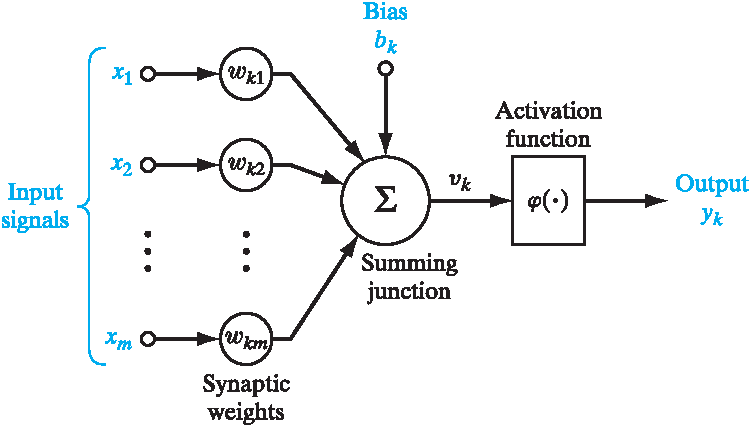
\includegraphics[width=0.8\linewidth]{figures/neuron.pdf}
    \addmargin
    \legend{Source: \citet{haykin2009neural}}
\end{figure}

Essentially, NNs are composed of multiple artificial neurons, whose structure is illustrated in \cref{fig:neuron}. A neuron~$k$ consists of four components: input signals~$x_1,\ldots,x_m$, weights~$w_{k1},\ldots,w_{km}$, bias term~$b_k$, and an activation function~$\varphi$. A neuron~$k$ produces an output~$y_k = \varphi(v_k + b_k)$ where $v_k = \sum_{j \in [m]} w_{kj} x_j$. The activation function introduces non-linearity to the output. One common example is the Rectified Linear Unit (ReLU) activation~$\varphi(v) = max(0,v)$.

\begin{figure}[tb]
    \caption[Graph of a neural network.]{Graph of a neural network. Vertices and edges represent the neurons and their connections, respectively.}
    \label{fig:neuralnetwork}
    \addmargin
    \centering
    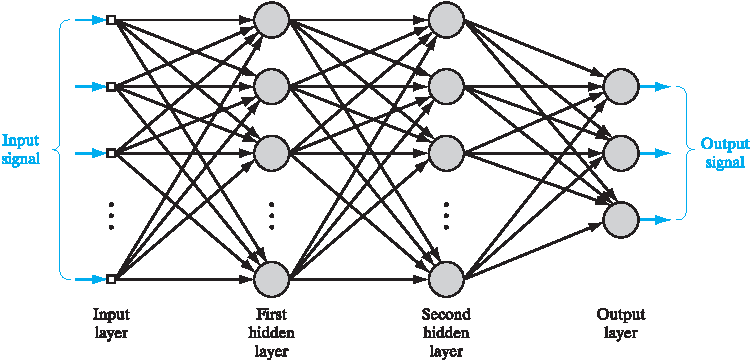
\includegraphics[width=0.9\linewidth]{figures/network.pdf}
    \addmargin
    \legend{Source: \citet{haykin2009neural}}
\end{figure}

The NN comprises multiple layers of neurons, as illustrated in \cref{fig:neuralnetwork}, which transform the input data into an output. The input layer receives the input data and passes it to the subsequent layers. The hidden layers, located between the input and output layers, weigh the neuron weights to learn the features that transform the input data into the desired output. These hidden layers enable the network to capture complex patterns and relationships within the data. Finally, the output layer produces the prediction for the given input. A specific type of NN called Feedforward Neural Network~(FNN) allows information to flow in one direction, from the input layer through the hidden layers to the output layer. When an NN has multiple hidden layers, usually more than two\rv{there is no consensus but it is common to find that, in general, more than two hidden layers is deep}, it is referred to as a deep neural network.

The learning process involves adjusting the network's parameters, such as weights and biases, to minimize the error between its predictions and the true values of the training samples. This adjustment is typically performed using an optimization algorithm to minimize a specified loss function. One commonly used loss function is the Mean Squared Error~(MSE), which quantifies the error by calculating the mean squared difference between the predicted and true values. Training is often performed on batches of data rather than individual samples to update the parameters efficiently. The batch size determines the number of samples that are processed together before updating the network's parameters. Batches enable training with larger sets of samples, which can be computationally infeasible to handle all at once. \citet{haykin2009neural} provides further details for a more comprehensive understanding of weight adjustment and training in NNs.

By iteratively adjusting its parameters based on the training data, an NN gradually improves its ability to make accurate predictions. The quality of the NN depends on the quality and diversity of the sample set. Additionally, the network's capacity to learn and generalize from the training data is influenced by its architecture. Each one has its purpose and may excel in specific types of tasks. One example of such an architecture is the residual network.

\subsection{Residual Networks}
\label{sec:resnets}

ResNet, short for Residual Network, was proposed by \citet{he2016deep} and has gained attention due to its ability to address the vanishing gradient problem~\cite{hochreiter1998vanishing} and improve training performance for deep NNs. While its initial success was in image recognition, ResNet has also been used in planning~\cite{agostinelli2019solving,ferber2022neural} to address training deep neural networks.

ResNet uses the concept of residual connections or skip connections, which enable the network to learn residual mappings. These connections allow the network to bypass specific layers and pass the input directly to deeper layers. By doing so, ResNet mitigates the vanishing gradient problem in deep networks, where the gradient becomes increasingly small as they propagate backward through the network layers, causing the weights in the earlier layers to update slowly or not at all. The residual connections establish ``highways'' for information flow, helping maintain the signal propagation.

\begin{figure}[tb]
    \caption[A regular block and a residual block.]{A regular block (left) and a residual block (right).}
    \label{fig:residual-block}
    \addmargin
    \centering
    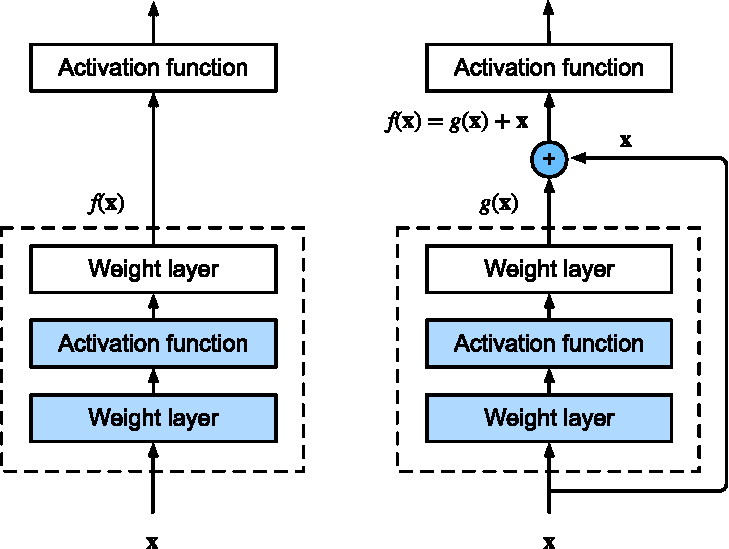
\includegraphics[width=0.75\linewidth]{figures/residual-block.pdf}
    \legend{Source: \citet{zhang2021dive}}
\end{figure}

\cref{fig:residual-block} illustrates a schematic representation of both a regular block and a residual block -- with a shortcut connection that skips two layers~-- in a ResNet architecture. In a regular block, the output of its layers is directly mapped to the activation function. On the other hand, in a residual block, the network needs to learn the residual mapping. Instead of forcing the network to learn all the information from the input, residual blocks allow it to focus only on the residual, i.e.,~the difference between the input and output, needed to achieve the desired output. \citet{he2016deep} provide a more detailed explanation of ResNets.

\subsection{Learning Heuristic Functions}
\label{sec:learning-heuristics}

Many heuristics for classical planning are derived from a model of the task, such as \sas. An obvious alternative is to learn to map a state~$s$ to its heuristic value~$h(s)$. We focus on learning with NNs, although other supervised learning methods could be used. To learn a heuristic function, an NN is trained on pairs of states~$s$ and cost-to-goal estimates~$c$. The learned heuristic functions are usually not admissible, so traditional optimality guarantees are lost.

A propositional representation of a state is more suitable for learning functions over states, as the variables in a planning task are categorical variables. To this end, consider a planning task~$\Pi=\langle\mathcal{V},\mathcal{O},s_0,s^*, \text{cost}\rangle$, and let $\mathcal{V}=\{v_1,\ldots,v_n\}$ and $D(v_i)=\{d_{i1},\ldots,d_{i,s_i}\}$, $i\in[n]$ be some order of the variables and their domains. We represent any state~$s$ by a sequence of facts $$\mathcal{F}(s)=(f_{11},f_{12},\ldots,f_{1,s_1},\ldots,f_{n1},f_{n2},\ldots,f_{n,s_n}),$$ where each fact~$f_{ij}=[s(v_i)=d_{ij}]$ indicates if variable~$v_i$ assumes value~$d_{ij}$ in state~$s$. Note that facts~$\mathcal{F}_i=\{f_{i1},\ldots,f_{i,s_i}\}$ corresponding to variable~$v_i$ satisfy the consistency condition~$\sum_{f\in \mathcal{F}_i} f\leq 1$ since each variable assumes at most one value, and $\sum_{f\in \mathcal{F}_i} f=0$ only if $v_i$ is undefined. More generally, for any set of facts~$\mathcal{F}$ we write $\mutex(\mathcal{F})$ if $\sum_{f\in \mathcal{F}} [f]\leq 1$ must be satisfied in states of $\Pi$. Many planning systems can deduce mutexes from the description of the planning task~$\Pi$~\cite{helmert2009concise}; we will discuss and analyze their utility for sampling states later. Some architectures provide additional input to the neural network, e.g.,~the propositional representation of the goal condition. The target output for training may be the cost-to-goal estimates directly or some encoding of them.

An important aspect of sample generation related to challenges C1 and C2~(\cref{chapter:introduction}) is the degree of dependency on the domain model -- ideally, we would like to learn in a model-free setting~-- or the planning task and the cost of generating the samples. The cost of sample generation depends on the number of samples and the cost to generate each. This generates the problem of deciding how many samples are required since, in general, only a very small part of the state space can be sampled. More importantly, ideal samples would be labeled with the optimal heuristic \hstar. In general, ideal labeling is impractical since it requires solving the planning task on a large number of initial states. Therefore, we are mainly interested in good heuristic estimates that can be generated fast. We analyze the influence of sample size and quality experimentally later.

Additionally, and related to challenges C3 and C4, network architecture and sample generation depend on the range of tasks the learner intends to generalize. This may be the state space of a planning task, a planning domain, or an entire planning formalism. In the first case, the set of planning tasks is defined over any pair of initial state~$s_0$ and goal~$s^*$. Often the set of planning tasks is restricted to select the initial state from the FSS of some given initial state and to a fixed goal. In the second case, the learned function has to generalize over all domain tasks. Finally, a learning-based heuristic that generalizes over a planning formalism is domain-independent. An important aspect of sample generation is the distribution of states which are part of the sample set. For example, the sample set can contain only states with a short distance to the goal or only states with a short distance to the initial states. In this dissertation, the distribution of \hstar-values, e.g.,~in a histogram, represents the distribution of states in the sample set.

\section{Related Work}
\label{sec:related-work}

Two main research topics have been on learning heuristic functions: strongly and partially model-based approaches. The first one uses model description, such as information about preconditions and effects of operators, to generate samples or build the NN and aims to generalize over domains or a planning formalism. The second one uses limited access to the model only to identify mutexes, generating states close to those encountered during a search, and aims to generalize only over a state space.

\subsection{Strongly Model-Based}
\label{sec:related-work-strongly}

The usual setting for the first set of approaches~\cite{toyer2018action,shen2020learning,toyer2020asnets,gehring2022reinforcement,stahlberg2022learning} is to train different architectures of NN with samples of small tasks of a domain generated with a strongly model-based method and evaluated on larger tasks of the same domain. These architectures can be general networks such as neural logic machines~\cite{dong2018neural} and graph neural networks~\cite{gori2005new,scarselli2008graph}.

In the context of planning, \citet{shen2020learning} introduced Hypergraph Neural Networks~(HGN) as an extension of graph networks~\cite{battaglia2018relational}. HGN aims to learn planning heuristics through training, focusing on developing domain-independent heuristics capable of generalizing across various domains, as well as domain-specific and multi-domain heuristics. The HGN encompasses vertices representing task propositions within a hypergraph structure, with edges denoting operators connecting the preconditions to their effects.

Another approach proposed explicitly for planning tasks is the Action Schema Networks~(ASNet)~\cite{toyer2018action}. ASNets are composed of alternating proposition and action layers, with the first and last always being an action layer. Each action layer contains an action module for each operator in a specific task, while each propositional layer contains a proposition module for each fact in the task. Weight sharing is used to optimize efficiency, where action modules with operators derived from the same action schema share the same weight, and proposition modules with atoms derived from the same predicate share the same weight. This weight sharing allows for the reuse of a single set of learned weights across all tasks within a class of planning problems.

These networks achieve competitive results compared to logic-based heuristics and can generalize well, but require the logical description of the domain and the task to be instantiated. These approaches also help in understanding learning heuristics. For example, the main goal of \citet{stahlberg2022learning} is to understand the expressive power and limitations of learning heuristics. The main limitation of these approaches is the strong dependence on the domain model and task description.

\subsection{Partially Model-Based}
\label{sec:related-work-partially}

The second set of approaches~\cite{ferber2020neural, yu2020learning, ferber2022neural, otoole2022sampling} typically trains an FNN and evaluates the learned heuristic on a state space using tasks with the same goal and different initial states. These networks are trained with pairs of states and cost-to-goal estimates. \citet{ferber2020neural} systematically study hyperparameters on the FNN and found that, for a fixed architecture, two aspects significantly influence how informed the heuristic is: the subset of selected samples and the size of the sample set.

\citet{ferber2022neural} use a combination of backward and forward searches~\cite{arfaee2011learning}. First, they generate new initial states with backward random walks and then solves them with a GBFS guided by a learned heuristic. The sampling is performed in parallel with the training. The number of samples per search varies throughout the process, starting with a random value ranging from $0$ to $5$ and doubling it as plans are found. The plans found provide the samples for the next training epoch, where each sample is a state in a plan with the cost-to-goal estimate as its distance to the goal through the plan. Their FNN architecture is a ResNet with two hidden layers and a residual block consisting of two more hidden layers.

\citet{otoole2022sampling} use the same FNN architecture as \citet{ferber2022neural}, which is also applied in this dissertation. They use random walks to perform $5$~backward searches from the goal, with a depth of~$500$, where the depth at which the state is generated serves as a cost-to-goal estimate. Each sampled partial state is then converted into $20$~complete states and added to the sample set. Furthermore, they sample an additional $50$\,K~randomly generated states with a cost-to-goal estimate equal to the maximum value in the sample set plus one, resulting in a total of $100$\,K~samples. They showed that random sampling improves the performance of the heuristic function by including in the sample set states from regions of the state space not reached by the backward search.

\citet{yu2020learning} used a backward search approach with the DFS algorithm. In their best configuration, they sample $100$\,K~states in $500$~searches, i.e.,~$200$~states per search, with a cost-to-goal estimate equal to the depth at which the state was generated. In contrast to the previous approaches, they use a compact FNN consisting of only one hidden layer with $16$~neurons.

The methods from the partially model-based approaches are highly independent of the domain model and planning task description and require low computational resources to generate samples and train the FNN. However, despite having competitive results compared to logic-based heuristics, they can still not surpass the goal-count heuristic.
